\documentclass[12pt]{article}
\usepackage[spanish]{babel}
\usepackage{natbib}
\usepackage{url}
\usepackage[utf8x]{inputenc}
\usepackage{amsmath}
\usepackage{float}
\usepackage{subfig}
\usepackage{graphicx}
\graphicspath{{images/}}
\usepackage{parskip}
\usepackage{fancyhdr}
\usepackage{vmargin}
\usepackage{mathtools}
\usepackage{amssymb} 



\title{Actividad \#10:Animaciones con Matplolib}							
\author{\Large Jesùs Valenzuela Nieblas\\}											
\date{\today} 

\makeatletter
\let\thetitle\@title
\let\theauthor\@author
\let\thedate\@date										
\makeatother

\pagestyle{fancy}

\lhead{\thetitle}
\cfoot{\thepage}
\rhead{}
\begin{document}

%%%%%%%%%%%%%%%%%%%%%%%%%%%%%%%%%%%%%%%%%%%%%%%%%%%%%%%%%%%%%%%%%%%%%%%%%%%%%%%%%%%%%%%%%

\begin{titlepage}
	\centering
    \vspace*{.5cm}
     
\includegraphics[scale = 0.7]{logo}\\	% University Logo
    \textsc{\Large Universidad de Sonora}\\[1.0 cm]	% University Name
	\textsc{\Large División de Ciencias Exactas y Naturales}\\[.50 cm]
  	\textsc{\Large Licenciatura en Fìsica}\\[.5 cm]
  \textsc{\large Fìsica Computacional 1}\\[1.5 cm]				% Course Name
	
	{ \huge \bfseries \thetitle}\\

    \vspace*{3 cm}
	\begin{minipage}{\textwidth}
    \centering
    \theauthor
	\end{minipage}\\[3 cm]
	
 
	\vfill
	
\end{titlepage}

%%%%%%%%%%%%%%%%%%%%%%%%%%%%%%%%%%%%%%%%%%%%%%%%%%%%%%%%%%%%%%%%%%%%%%%%%%%%%%%%%%%%%%%%%

\section{Introducciòn}
Para poder apreciar si la simulación está funcionando correctamente, lo mejor que puede hacerse es visualizar la forma en que está evolucionando a través de gráficas y animaciones.\\
Matplotlib es una biblioteca para la generación de gráficos a partir de datos contenidos en listas o arrays en el lenguaje de programación Python y su extensión matemática NumPy. Proporciona una API, pylab, diseñada para recordar a la de MATLAB.



\section{Código}
\begin{verbatim}

# coding: utf-8

# In[ ]:

from numpy import sin, cos
import numpy as np
import matplotlib.pyplot as plt
import scipy.integrate as integrate
import matplotlib.animation as an
from matplotlib.lines import Line2D
from scipy.integrate import odeint

class DoublePendulum:
    def __init__(self,
                 init_state = [0, 0, 0, 0],
                 L1 = 1.0,  # Longitud del pendulo 1
                 L2 = 0.0,  # Longitud del pendulo 2
                 M1 = 1.0,  # Masa del pendulo 1
                 M2 = 1.0,  # Masa del pendulo 2
                 G = 9.8,   # Aceleracion por la gravedad
                 origin=(0, 0)): 
        self.init_state = np.asarray(init_state, dtype='float')
        self.params = (L1, L2, M1, M2, G)
        self.origin = origin
        self.time_elapsed = 0

        self.state = self.init_state * np.pi / 180.
    
    def position(self):
        (L1, L2, M1, M2, G) = self.params

        x = np.cumsum([self.origin[0],
                       L1 * sin(self.state[0]),
                       L2 * sin(self.state[2])])
        y = np.cumsum([self.origin[1],
                       -L1 * cos(self.state[0]),
                       -L2 * cos(self.state[2])])
        return (x, y)

    def energy(self):
        (L1, L2, M1, M2, G) = self.params

        x = np.cumsum([L1 * sin(self.state[0]),
                       L2 * sin(self.state[2])])
        y = np.cumsum([-L1 * cos(self.state[0]),
                       -L2 * cos(self.state[2])])
        vx = np.cumsum([L1 * self.state[1] * cos(self.state[0]),
                        L2 * self.state[3] * cos(self.state[2])])
        vy = np.cumsum([L1 * self.state[1] * sin(self.state[0]),
                        L2 * self.state[3] * sin(self.state[2])])

        U = G * (M1 * y[0] + M2 * y[1])
        K = 0.5 * (M1 * np.dot(vx, vx) + M2 * np.dot(vy, vy))

        return U + K

    def dstate_dt(self, state, t):
        (M1, M2, L1, L2, G) = self.params

        dydx = np.zeros_like(state)
        dydx[0] = state[1]
        dydx[2] = state[3]

        cos_delta = cos(state[2] - state[0])
        sin_delta = sin(state[2] - state[0])

        den1 = (M1 + M2) * L1 - M2 * L1 * cos_delta * cos_delta
        dydx[1] = (M2 * L1 * state[1] * state[1] * sin_delta * cos_delta
                   + M2 * G * sin(state[2]) * cos_delta
                   + M2 * L2 * state[3] * state[3] * sin_delta
                   - (M1 + M2) * G * sin(state[0])) / den1

        den2 = (L2 / L1) * den1
        dydx[3] = (-M2 * L2 * state[3] * state[3] * sin_delta * cos_delta
                   + (M1 + M2) * G * sin(state[0]) * cos_delta
                   - (M1 + M2) * L1 * state[1] * state[1] * sin_delta
                   - (M1 + M2) * G * sin(state[2])) / den2
        
        return dydx

    def step(self, dt):
        self.state = integrate.odeint(self.dstate_dt, self.state, [0, dt])[1]
        self.time_elapsed += dt

#-----------------------
#CI para el pendulo
theta0=35
v0= 20
pendulum = DoublePendulum([theta0, v0, 0.0, 0.0])

#-----------------------
#CI para el espacio fase
g = 9.81 #valor de g
l = 1.0 #longitud
b = 0.0 #no friccion
c = g/l

X_f1 =np.array([(theta0/180.0)*np.pi,(v0/180.0)*np.pi])
t = np.linspace(0,30,500)

#ED del pendulo
def p (y, t, b, c):
    theta, omega = y
    dy_dt = [omega,-b*omega -c*np.sin(theta)]
    return dy_dt

#Trayectoria
y0 = X_f1                       
X = odeint(p, y0, t, args=(b,c))         

#-----------------------
#Animacion del pendulo
dt = 1./60.
fig = plt.figure()
ax = fig.add_subplot(111, aspect='equal', autoscale_on=False,
                     xlim=(-2, 2), ylim=(-2, 2))
ax.grid()

line, = ax.plot([], [], 'o-', lw=2, color='r')
time_text = ax.text(0.02, 0.95, '', transform=ax.transAxes)
energy_text = ax.text(0.02, 0.90, '', transform=ax.transAxes)

def init():
    #iniciando animacion
    line.set_data([], [])
    time_text.set_text('')
    energy_text.set_text('')
    return line, time_text, energy_text

def animate(i):
    #animar las fotitos
    global pendulum, dt
    pendulum.step(dt)
    line.set_data(*pendulum.position())
    return line, time_text, energy_text

from time import time
t0 = time()
animate(0)
t1 = time()
interval = 1000 * dt - (t1 - t0)

ani = an.FuncAnimation(fig, animate, frames=300,
                              interval=interval, blit=True, init_func=init)
plt.show()

class SubplotAnimation(an.TimedAnimation):
    def __init__(self):
        fig = plt.figure()
        ax1 = fig.add_subplot(1, 1, 1)
       
        self.t = np.linspace(0, 80, 400)
        self.x = X[:,0]
        self.y = X[:,1]

        self.line1 = Line2D([], [], color='y')
        self.line1a = Line2D([], [], color='g', linewidth=2)
        self.line1e = Line2D(
            [], [], color='g', marker='o', markeredgecolor='r')
        ax1.add_line(self.line1)
        ax1.add_line(self.line1a)
        ax1.add_line(self.line1e)
        ax1.set_xlim(-10, 10)
        ax1.set_ylim(-10, 10)
        ax1.grid()
        ax1.set_aspect('equal', 'datalim')

        an.TimedAnimation.__init__(self, fig, interval=50, blit=True)

    def _draw_frame(self, framedata):
        i = framedata
        head = i - 1
        head_slice = (self.t > self.t[i] - 1.0) & (self.t < self.t[i])

        self.line1.set_data(self.x[:i], self.y[:i])
        self.line1a.set_data(self.x[head_slice], self.y[head_slice])
        self.line1e.set_data(self.x[head], self.y[head])

    def new_frame_seq(self):
        return iter(range(self.t.size))

    def _init_draw(self):
        lines = [self.line1, self.line1a, self.line1e]
        for l in lines:
            l.set_data([], [])

ani = SubplotAnimation()
plt.show()
ani.save('double_pendulum.mp4', fps=30, extra_args=['-vcodec', 'libx264'])

#-----------------------





\end{verbatim}

\section{Gráficas}
\subsection{ Para 0 grados}
\begin{figure}[H]
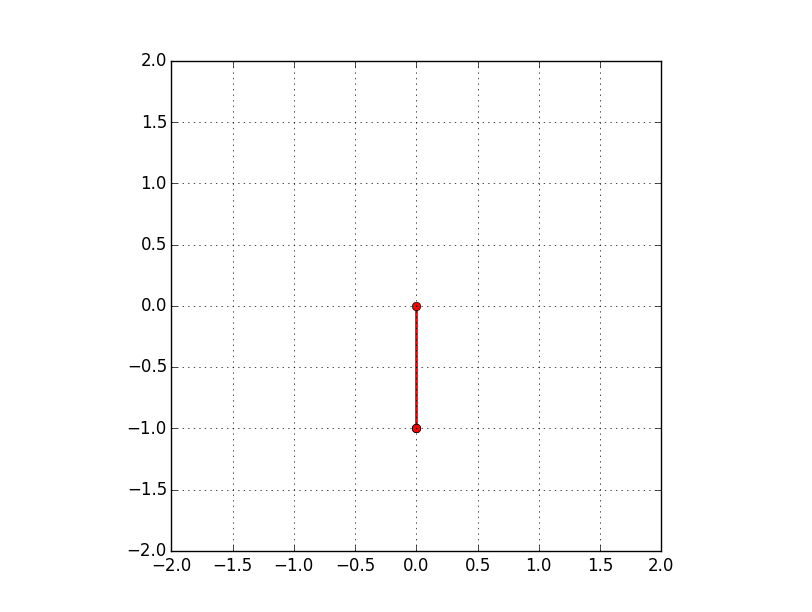
\includegraphics[scale=.6]{0p}
\end{figure}
\begin{figure}[H]
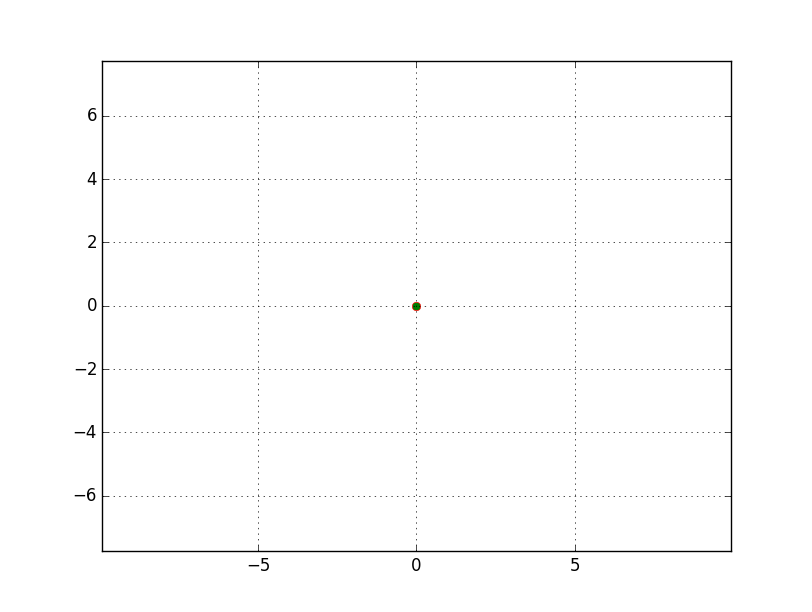
\includegraphics[scale=.6]{0e}
\end{figure}


\subsection{Para 35 grados}
\begin{figure}[H]
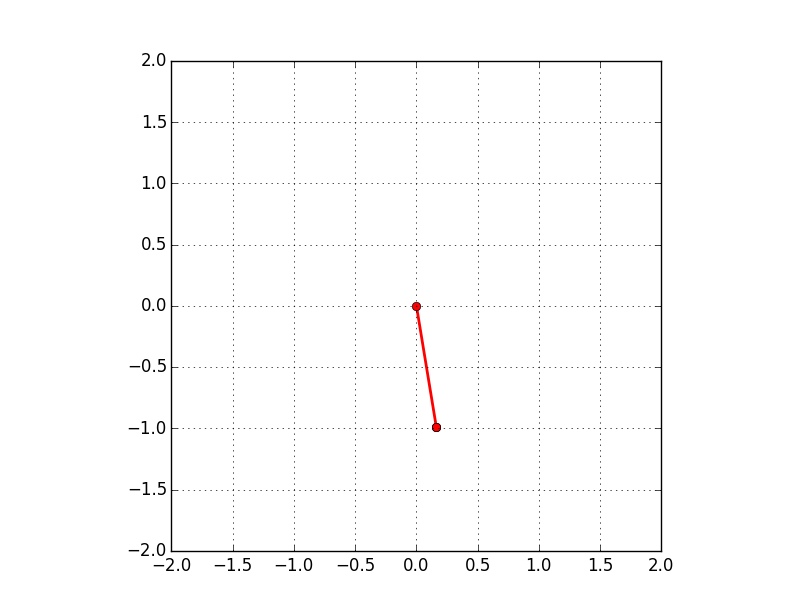
\includegraphics[scale=.6]{35p}
\end{figure}
\begin{figure}[H]
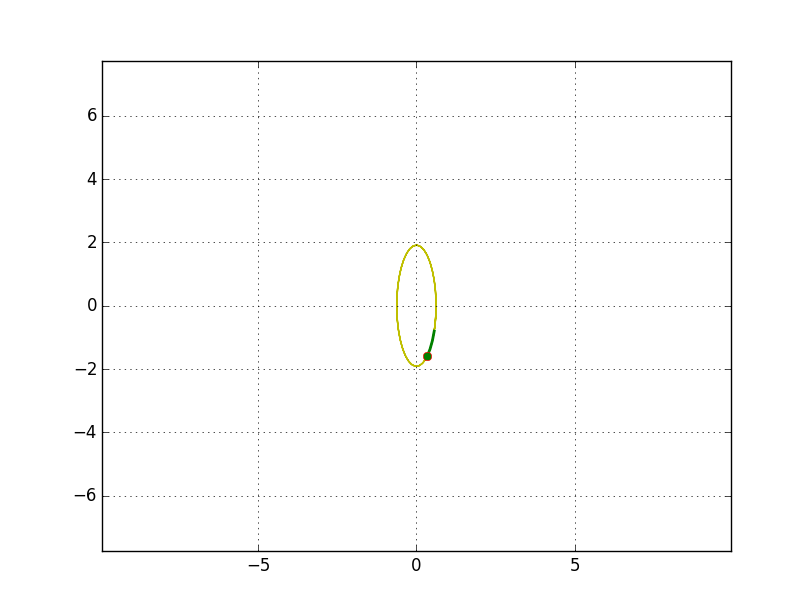
\includegraphics[scale=.6]{35e}
\end{figure}

\subsection{para 90 grados}
\begin{figure}[H]
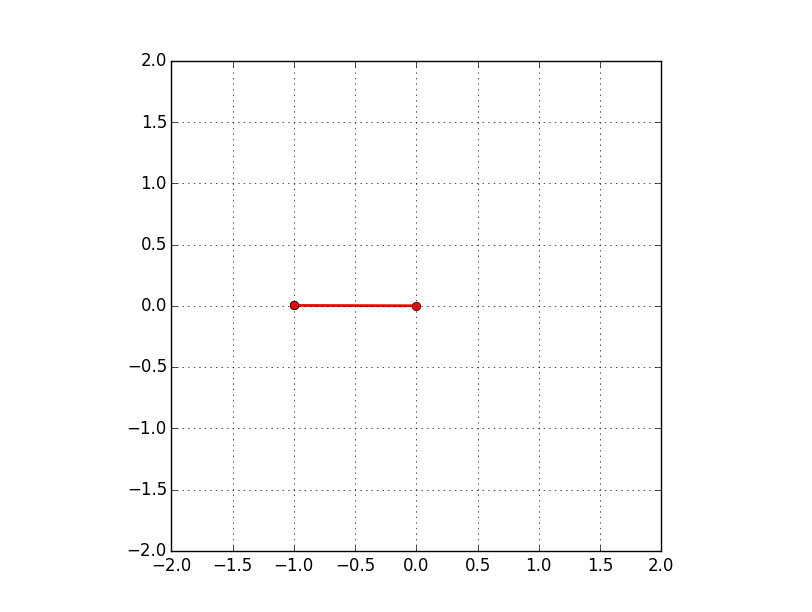
\includegraphics[scale=.6]{90p}
\end{figure}
\begin{figure}[H]
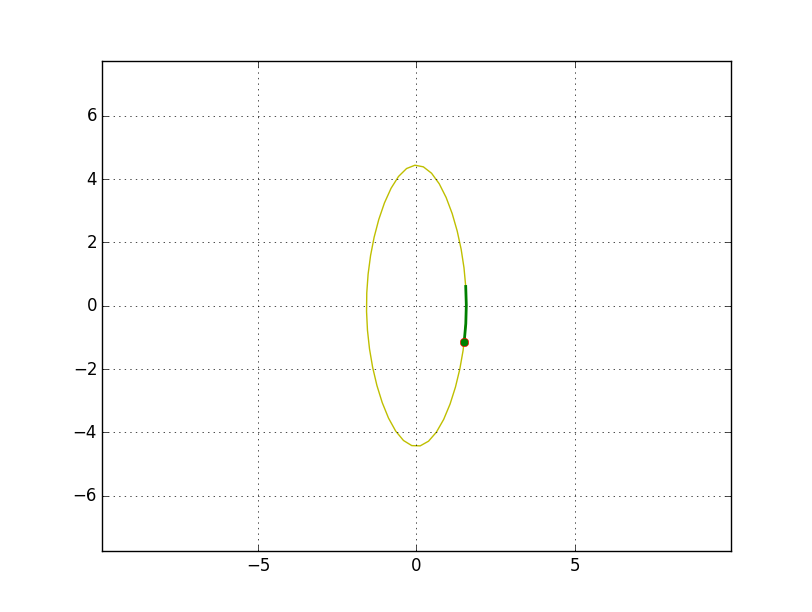
\includegraphics[scale=.6]{90e}
\end{figure}

\subsection{Para 135 grados}
\begin{figure}[H]
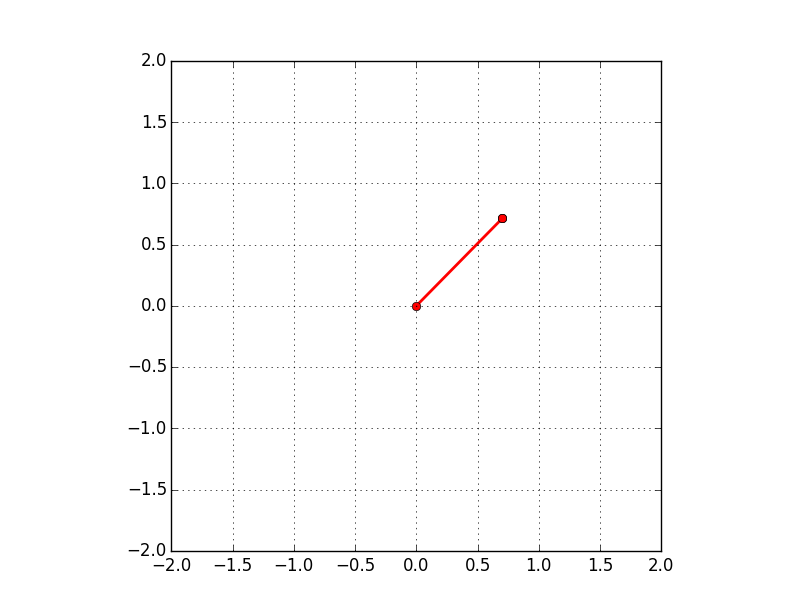
\includegraphics[scale=.6]{135p}
\end{figure}
\begin{figure}[H]
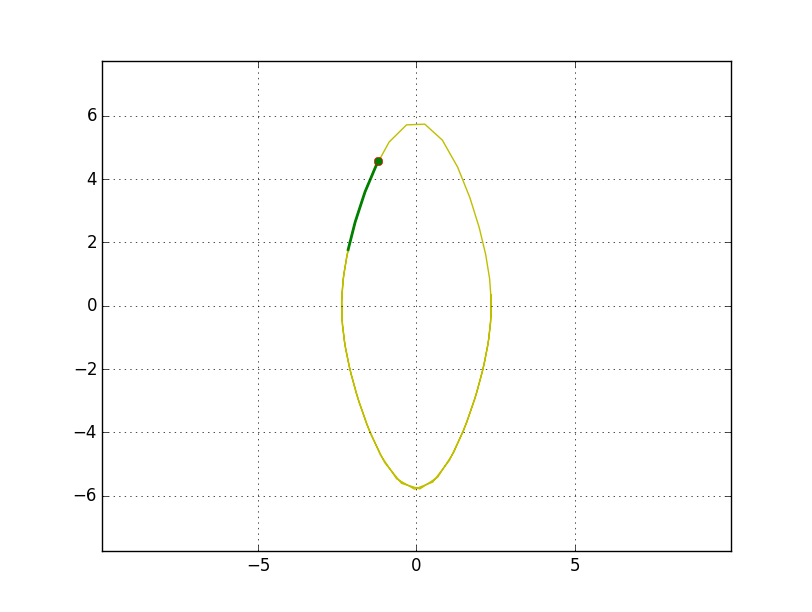
\includegraphics[scale=.6]{135e}
\end{figure}

\subsection{Para 170 grados}
\begin{figure}[H]
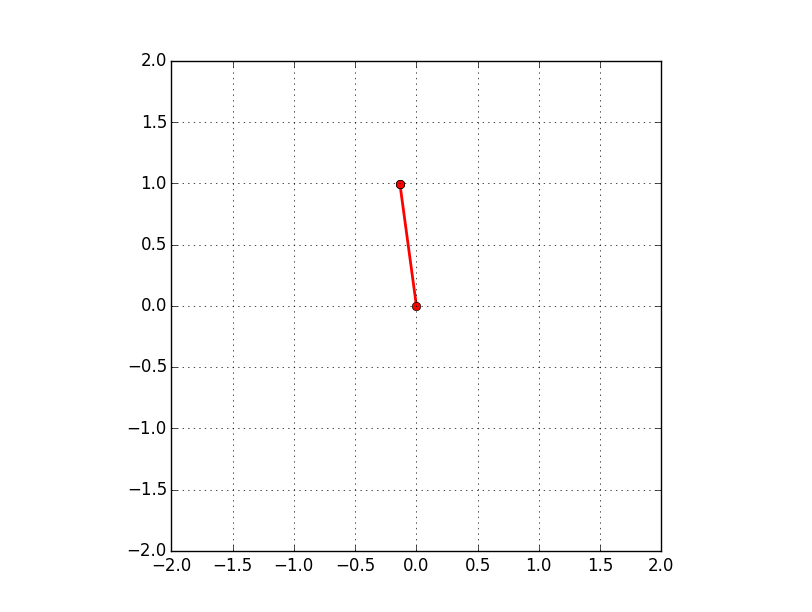
\includegraphics[scale=.6]{170p}
\end{figure}
\begin{figure}[H]
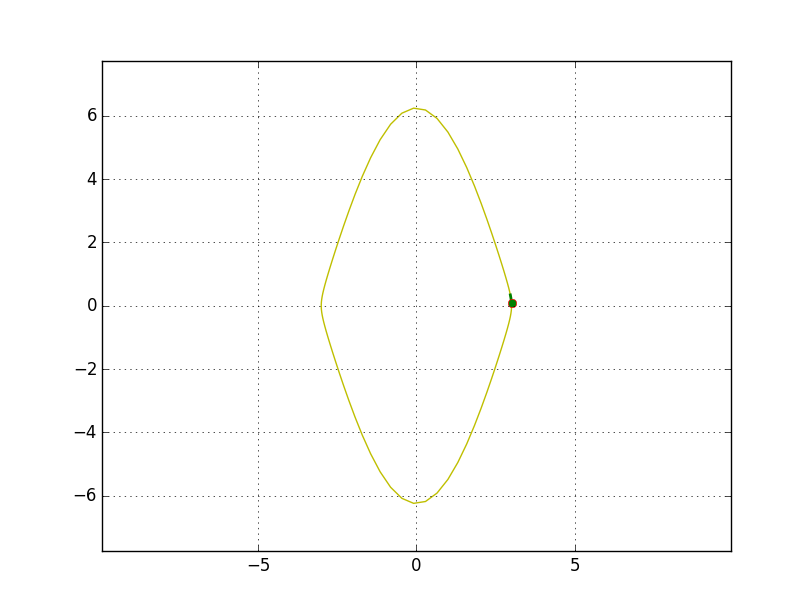
\includegraphics[scale=.6]{170e}
\end{figure}

\subsection{Para 180 grados}
\begin{figure}[H]
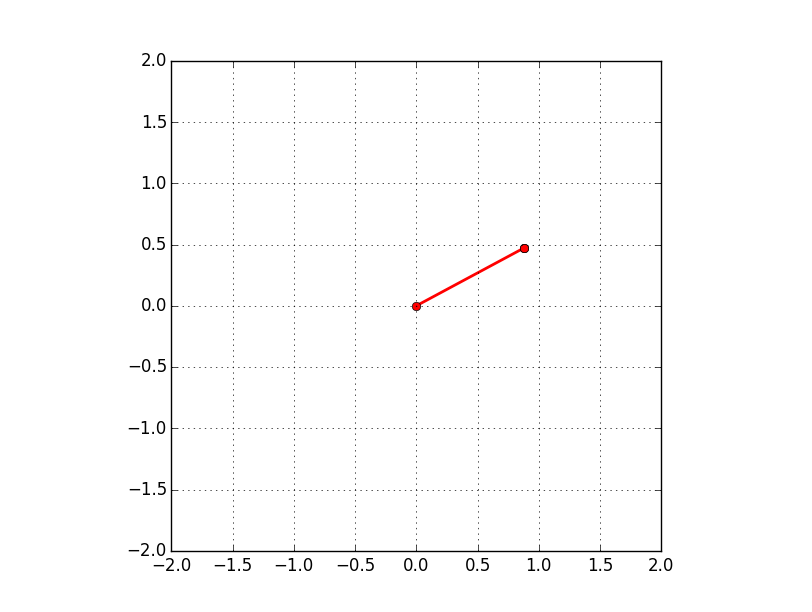
\includegraphics[scale=.6]{180p}
\end{figure}
\begin{figure}[H]
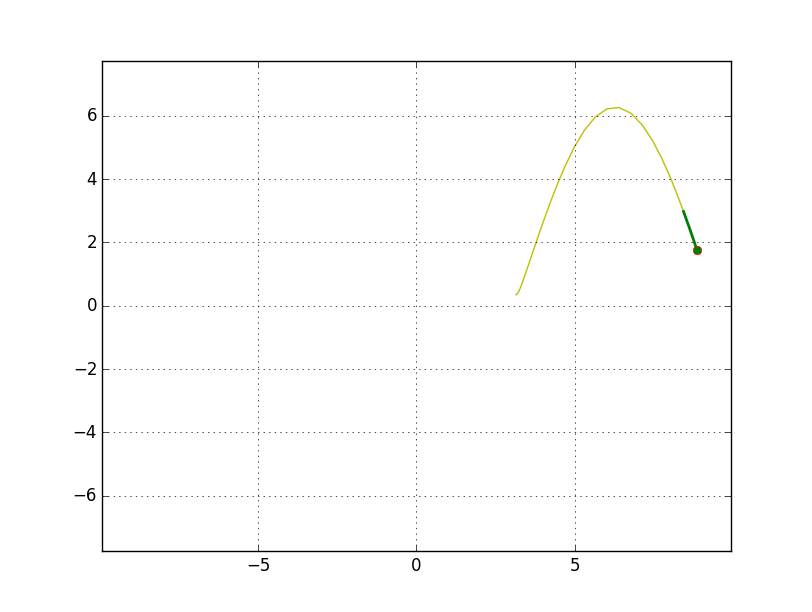
\includegraphics[scale=.6]{180e}
\end{figure}
\end{document}
